\chapter{Approach- state HYPOTHESIS AND ASSUMPTIONS LIKE YOU SAW, DON'T SAY ANYTHING FOR SURE!!  } % Main chapter title
\addtocontents{toc}{\protect\setcounter{tocdepth}{1}}
\label{Chapter3} % For referencing the chapter elsewhere, use \ref{Chapter1} 

\lhead{Chapter 5. \emph{Approach}}

This chapter presents the scope and approach behind the research questions raised earlier and develops a set of metrics for answering these questions.

\section{Challenges of Selenium Test Automation}
\label{challengesSelenium}
The purpose of test automation using Selenium framework is to spare the time and effort involved in executing regression tests manually. However, as with every test automation techniques, test automation with Selenium has its own limitations. This section gives a brief overview about the commonly faced challenges in Selenium testing.

Selenium tests are broken if certain functionalities are modified or the order in which the functionality has to be accessed is altered.
Such changed functionality cannot be covered by the existing tests unless the tests are modified, since the same test inputs can lead to different application behavior. Tests can encounter failures when certain assumptions or preconditions required for them to execute become invalid, such as loading the application to a particular \textit{initial state}.

If a single test case attempts to cover more than one functionality through multiple steps, a failure during initial steps can result in following test not being able to reach the subsequent functionality.

Modifying the structural markup and GUI elements of a web page can affect the performance of the tests. Selenium tests can be broken if the manner in which a functionality is accessed (such as clickable objects, buttons, forms etc.) is modified. Moreover, if GUI element locators (e.g. \texttt{id, xpath, css selectors} etc.) are changed or incorrectly selected, the test cases might be unable to find the object on the page as these attributes can no longer be valid.

Depending upon various factors, different pages of the AUT can load with different speeds. If not load properly, Selenium tests would not be able to explore the desired web page. Moreover, server side requests such as Ajax and JavaScript calls can contribute towards random loading times. Recognizing when such calls are finished can be intricate for Selenium \texttt{webdriver} API. Network latency, bandwidth bottlenecks and database related issues can also result in delayed, improper or partial loading of the AUT state. Such problems can make the tests fail due to the unavailability of certain objects.

Flash related objects are rendered as closed files encompassed in a container and are not accessible using the likes of \texttt{xpath} or \texttt{HTML} based element locators. Selenium \texttt{webdriver} itself has no direct interface to interact with such content. 

In order to detect and mitigate the aforementioned issues, different problems may need different methods. Within the scope of this research, it might not be possible to detect non-deterministic and sporadic failures occurring due to server side problems, random timing issues, network latency etc. which are difficult to reproduce or to analyze. Moreover, our approach will not be able to cover Flash-related functionality due to the limitations inherited from Selenium \texttt{webdriver} itself.

On the other hand, the approach presented in this thesis is suitable for the identification of the most important factors contributing towards the robustness of Selenium tests, such as the design of the test-suite, choice of GUI element locators, number of steps executed by the test etc. In the subsequent sections, details of our approach are presented as follows -- Section \ref{robustnessOfSeleniumTests} develops the concept of robustness in the area of Selenium testing and formally introduces the metric \textit{robustness grade}. The metrics for the assessment of the most important factors contributing towards the \textit{robustness}, namely the design and composition of the test-suite are presented in Section \ref{robfactors}. The effort required to repair a test-suite according to the changes in the AUT can also given an indication of its robustness. Section \ref{locatorMaintenance} discusses the effect of test-suite's design considerations on its maintenance. 

\section{Robustness of Selenium Tests (RQ1)}
\label{robustnessOfSeleniumTests}
% This section explains the notion behind robustness of Selenium tests and introduces the metric for measuring the robustness over different software revisions.

% Selenium tests are robust if they can cover (explore) the same functionality even as the AUT changes over time.  
% In practice, however, the robustness of a test decreases over time and the tests needs to be maintain as the application evolves, as mentioned in Chapter \ref{Chapter1}. 
The primary objective of thesis is to assess how robust Selenium tests are against the changes in the application. As a starting point, it is essential to define the \textit{robustness} of Selenium tests. 

Within the scope of this thesis, the \textit{robustness} of a Selenium test considers the degree of its stability and effectiveness to cover the intended functionality across different versions of the AUT. A robust test covers the same functionality across different revisions of the AUT and in cases where it fails, possible software \textit{regression} related to that functionality is found. Intuitively, if a test is robust against the changes in the AUT, it does not need to be constantly repaired.

% Triggering certain behavior can involve multiple underlying functionalities and layers such as input validation, database operations etc.
% When the GUI of the application evolves over time, it usually evolves with other layers as opposed to changing in a standalone manner. As a result, the success of a test to cover the same functionality each time the application evolves depends on changes in other layers as well.
% As an example, consider the \textit{click `Login' button} scenario from the \texttt{loginTest} in Listing \ref{code1}. If the new changes in AUT delays the time required for the GUI element locator of \textit{`Login'} button to be available in the DOM, the \texttt{loginTest} can fail randomly due to timing issues. Without specifying additional \texttt{wait} conditions in the test, 


  

% A test-suite is robust if it is able to cover the same functionality as the application changes over time.  

When developing automated tests, usually a test-suite (\textit{TS}) comprising several tests (\textit{$T_1$,$T_2$..,$T_n$}) is developed for some \textit{base version} (\textit{$V_{0}$}) of the AUT. This test-suite is then modified and maintained over time according to the changes in AUT. Farther the AUT evolves from the \textit{base version}, the lesser number of tests still remain robust. To evaluate how robust any test \textit{T} is over time, it is important to measure whether the test is able to cover the same functionality across different versions of AUT. As mentioned in Chapter \ref{Chapter2}, such a functionality coverage can be captured in terms of behavioral state models \cite{marchettoStateBased}, \cite{SchurMiningBehavModels}. If a test execution on different application versions results the same states of the behavioral model, such test can be considered robust.

Our approach proposes to measure the robustness of test \textit{T} for a \textit{new version $V_{1}$} of the AUT against a \textit{reference version} \textit{$V_{0}$}. The \textit{reference version} of the AUT is the \textit{base version} for which the test \textit{T} is originally written and the states (functionalities) covered by \textit{T} are identified. The \textit{new version} corresponds to an iterative revision of the AUT. The approach is straightforward -- the result of executing \textit{T} on reference version \textit{$V_{0}$} acts as a \textit{comparative oracle}, a benchmark against which performance of \textit{T} on new version \textit{V$_{1}$} can be measured. Formally, we define the \textit{
robustness grade} (Definition \ref{test-case-robustness}) to determine the robustness of Selenium tests. 

% Robustness equation%
\theoremstyle{definition}

\begin{definition}{The \textit{robustness grade} $R_{T_{V_{0}V_{1}}}$ of test \textit{T} for version \textit{$V_{1}$} compared against the reference version \textit{$V_{0}$} is as follows:}
\begin{center}
\vspace{0.5cm}
$(R_{T_{V_{0}V_{1}}}) = \displaystyle \frac{\#\thinspace of \thinspace same \thinspace states \thinspace reached \thinspace for \thinspace V_{1} \thinspace using \thinspace \thinspace T}{\# \thinspace of \thinspace same \thinspace states \thinspace reached  \thinspace for \thinspace V_{0} \thinspace using \thinspace \thinspace T}$ \normalsize
\end{center}
\label{test-case-robustness} 
% \vspace{0.5cm}
\end{definition} 

As a starting point, we assume that the state extraction points for the reference version as well as subsequent versions remain the same as the test-suites remain unchanged. Consequently, \textit{
robustness grade} lies in the interval [0,1]. A value of \textit{
robustness grade} equal to one ($R_{T_{V_{0}V_{1}}}=1$) indicates that the test covers same functionality across versions \textit{$V_{0}$} and \textit{$V_{1}$}. A value other than one ($R_{T_{V_{0}V_{1}}}\neq 1$) indicates that the test is not robust, as it does not cover same states across two different versions. The details of our approach to identify the states reached and functionalities covered across different versions are explained in Chapter \ref{Chapter4}.

Additionally, it would be interesting to know the \textit{
robustness grade} at test-suite level. Correspondingly, Definition \ref{test-suite-robustness} formulates the \textit{
robustness grade} for a test-suite.

\theoremstyle{definition}
\begin{definition}{The \textit{robustness grade} $R_{TS_{V_{0}V_{1}}}$ for test-suite \textit{TS} comprising \textit{n} tests (\textit{$T_1$,$T_2$..,$T_n$}) and executed on version \textit{$V_{1}$} is as follows:}
\vspace{0.5cm}
\begin{center}
$(R_{TS_{V_{0}V_{1}}}) = \displaystyle \frac{\#\thinspace of \thinspace robust \thinspace tests \thinspace for \thinspace V_{1} \thinspace using \thinspace \thinspace TS}{\# \thinspace of \thinspace robust \thinspace tests \thinspace for  \thinspace V_{0} \thinspace using \thinspace \thinspace TS}$ \normalsize
\end{center}
\label{test-suite-robustness}
\end{definition}

If the result of executing \textit{TS} on \textit{$V_{1}$} yields the same number of robust tests as it does for \textit{$V_{0}$}, test-suite \textit{TS} is fully robust ($R_{TS_{V_{0}V_{1}}} =1$). On the contrary, \textit{
robustness grade} less than one ($R_{TS_{V_{0}V_{1}}} < 1$) deems that one or more tests in \textit{TS} are not be fully robust and that the test-suite might be unable to cover the same application behavior for different versions. 

For measuring the robustness of Selenium tests, our approach considers two kinds of versions of the AUT, as follows: (i) major versions (stable releases) where significant changes are made in the functionality of the AUT and (ii) minor revisions (e.g. commits to the version control repository) where minor feature changes and bug fixes have been implemented. Throughout this thesis, the major versions of the AUT are treated as a \textit{reference versions} against which robustness of Selenium tests for software revisions (minor versions) is compared. 

% In a traditional software development environment, there can be multiple minor revisions for each major version. 

As web applications evolve from one revision to another, it is essential to assess how far in the development cycle does the test become fragile. By determining the robustness of a Selenium test across multiple revisions of a major release, it is possible to assess how robust the test remains from the time it was developed. This is formally expressed in Definition \ref{robustness-ground-truth}. 

% Robustness equation%
\theoremstyle{definition}

\begin{definition}{The \textit{
robustness grade} ${R_{T_{V_1,...,V_n}}}$ of test \textit{T} across \textit{n} minor versions \textit{$V_1,...,V_n$} of major version \textit{$V_{0}$} is calculated as follows:}
\begin{center}
\vspace{0.5cm}
${R_{T_{V_1,...,V_n}}} = \displaystyle \frac{R_{T_{V_{0}V_{1}}} + R_{T_{V_{0}V_{2}}} + ... + R_{T_{V_{0}V_{n}}}}{n}$ \normalsize
% \vspace{3cm}
\newline
\newline
\newline
% \textit{$R_{T_{V_{0}V_{1}}},..,R_{T_{V_{0}V_{n}}}$ = \textit{
% robustness grades} of \textit{$V_1,...,V_n$}} (see Definition \ref{test-case-robustness})
\end{center}
\label{robustness-ground-truth}  
% \vspace{0.5cm}
\end{definition} 
% The rationale behind this approach is that because there can be significant functionality changes between different major versions, there exists different versions of Selenium test-suites for different major versions.

%### GROUND TRUTH
% \begin{equation}
% robustness \thinspace ground\thinspace  truth\thinspace  (R_{T_{V_{0}V_{1}}}) = \displaystyle \frac{\#\thinspace of \thinspace same \thinspace states \thinspace reached \thinspace for \thinspace V_{1} \thinspace using \thinspace \thinspace T}{\# \thinspace of \thinspace same \thinspace states \thinspace reached  \thinspace for \thinspace V_{0} \thinspace using \thinspace \thinspace T}\normalsize
% \label{test-case-robustness}
% \vspace{0.5cm}
% \end{equation}

Where, \textit{$R_{T_{V_{0}V_{1}}},..,R_{T_{V_{0}V_{n}}}$} are the 
\textit{robustness grades} of \textit{$V_1,...,V_n$} according to Definition \ref{test-case-robustness}. The \textit{robustness grade} ${R_{T_{V_1,...,V_n}}}$ of a test over all minor versions lies in the interval [0,1]. A value equal to one (${R_{T_{V_1,...,V_n}}}=1$) indicates that the test is fully robust across all minor versions. This step establishes the \textit{ground truth} for the robustness analysis. 

Using the metric \textit{robustness grade} at test as well as at test-suite level (Definitions \ref{test-case-robustness}, \ref{test-suite-robustness}, \ref{robustness-ground-truth}), it is now possible to quantitatively measure how robust Selenium tests are against the changes of the AUT. 

\section{Design and Composition of Tests (RQ2)}
\label{robfactors}
There are various \textit{building blocks} that compose a Selenium \texttt{webdriver} based test, which are described in Section \ref{testDesignPractices}. This composition can be broadly classified into GUI element locators and various \textit{actions} performed by the test on the underlying application. Since different test can have different set of \textit{building blocks}, it would be beneficial for the developers to know whether the the manner in which the test-suite is constructed, such as the type and distribution of the these blocks test-suites affects the robustness of the tests. This section presents the metrics for determining whether there is a relation between these building blocks and robustness of Selenium tests.  

\subsection{Actions Executed by Tests}
\label{test-actions}
The \texttt{webdriver} API offers a rich set of \textit{actions} to be emulated on the AUT. The actions are a sequence of GUI events executed by the test on the AUT. These actions can be classified into state-changing actions, assertions and requesting additional information about the AUT, such as page resources. 

As the number of actions increases, the number of GUI sequences increases as well. A test performing a multitude of GUI sequences can attempt to cover \textit{too much} of functionality. Consider an example when a single test is written to test two functionalities -- if it succeeds in covering one of the functionality but fails to cover the other one, the test is broken. This can be a bad sign for its robustness. 
% Consider an example when a test-case is required to test whether an administrative user can access certain administrative privilege (such as adding new users). The test-case should not be required to test additional functionality, such as first creating an administrative user and then testing the administrative privileges. 
The number of actions executed by a test can be an indication of how \textit{atomic} the test is. Table \ref{rq2metrics} represents the number of actions \textit{\#actions} as a robustness metric. 

Recalling from Section \ref{sssec:emulatingActions}, a state-changing action such as a \texttt{click} event or a \texttt{get} request to a URL\footnote{Uniform Resource Locator} causes the AUT to load into a new state (e.g. new web page). After loading the AUT to a new state, a next action can be executed by the test. Consider the versatile \texttt{click} action as an example -- a \texttt{click} action can be used on various GUI elements, such as buttons, check-boxes, drop-down lists etc. Due to such versatility, triggering a \texttt{click} event on the AUT can invoke multiple underlying functionality layers such as input validation, database operations etc. A \texttt{get} request navigates the AUT to a web page, which might involve steps such as starting the browser window, loading the web page etc. Although Selenium \texttt{webdriver} provides the possibility of setting page loading times, it introduces additional delays. Nevertheless, after the state-changing actions the AUT needs to have all the GUI elements present before executing the next action. If the new state of the application is not loaded in a timely manner or not loaded at all, the next action would not be executed, and as a result the test is broken. In this manner as the number of state-changing actions can affect the robustness of a test. Table \ref{rq2metrics} represents these two metrics as \textit{\#gets} and \textit{\#clicks}.

Text input testing with Selenium, e.g. form filling, involves multiple actions on the AUT such as locating the input field, sending input to the field (e.g. using \texttt{sendKeysToElement} command) and submitting the input data. Different text input fields can have different requirements for the input type. A telephone number input field might not allow any letters. Multilingual websites using \textit{localization} can have different input restrictions depending upon the locale. According to the input field, each test can require specific mechanism to verify the correctness of the input text. This process is further complicated with web 2.0 applications using Ajax and JQuery technologies. Text fields with \textit{autocomplete} feature can rely on dynamically created DOM elements. To avoid race conditions, a \texttt{webdriver} test needs to make assure that the element is initialized before clicking. Due to the sheer number of possible input combinations, form data submission using Selenium is not trivial and can significantly influence the robustness of Selenium tests. The number of text inputs as a robustness metric is expressed as \textit{\#textInputs} in Table \ref{rq2metrics}. 
\begin{center}
\begin{table}
\centering
\resizebox{10cm}{!}{
\begin{tabular}{l*{6}{l}r}
\hline
Robustness Metric              &Description \\
\hline
\textit{\#actions} & Total number of \textit{actions} on AUT \\
\textit{\#gets}      & Number of \texttt{get} requests\\
\textit{\#textInputs} & Number of text inputs   \\
\textit{\#clicks}     & Number of \texttt{click} actions  \\
\hline
\textit{\#waits}    & Number of \texttt{wait} requests   \\
\hline
\textit{\#xpath}    & Number of \texttt{xpath} locators \\
\textit{\#partialLinkText}    & Number of \texttt{partial link text} locators  \\
\textit{\#className}    & Number of \texttt{class name} locators  \\
\textit{\#linkText}    & Number of \texttt{link text} locators   \\
\textit{\#name}    & Number of \texttt{name} locators  \\
\textit{\#cssSelector}    & Number of \texttt{css selector} locators  \\
\textit{\#tagName}    & Number of \texttt{tag name} locators   \\
\textit{\#id}    & Number of  \texttt{id} locators  \\
\hline
% \caption{Application Candidates}
\end{tabular}}
\captionsetup{justification=justified,
singlelinecheck=false}
\caption{Overview of the robustness metrics of a test. The first part represents the number of actions executed by the test, the second part represents the number of \texttt{wait} conditions in the test, the third part represents the number of GUI element locator requests in the test.}
\label{rq2metrics}
\end{table}
\end{center}
% AJAX Scripts - send a first key - get an image sayign your pw is weak, credit card numbers. Form data validation is a severe part of web testing. Complexity of form filling are thoroughly tested. 
% Consider a state-changing action -- the \textit{click `Login' button} scenario from the \texttt{loginTest} in Listing \ref{code1}. Recalling from Section \ref{sssec:emulatingActions}, a state-changing action causes the AUT to load into some \textit{next state} (e.g. new web page) on which some \textit{next action} can be executed. Triggering this \textit{click} event can invoke multiple underlying functionality layers such as input validation, database operations etc.
% Nevertheless, after the \textit{click} event the AUT needs to load all the GUI element so that the test can execute the \textit{next action}. If the \textit{next state} of the application is not loaded in a timely manner or not loaded at all, \textit{next action} would not be executed, and as a result the test is broken. In this manner, given next action higher the number of state-changing actions a test executes, the more probability of it being fragile. This metric is formally expressed as number of \textit{actions}
\subsection{Wait Conditions in Tests}
\label{selenium-waits-metric}
The Selenium \texttt{webdriver} API provides the possibility to insert \texttt{wait} conditions in the tests, as mentioned in Section \ref{sssec:seleniumwaits}. The \texttt{wait} commands can be used as a method for synchronizing between the action performed by the test and the response received from the \texttt{webdriver}. If the AUT implements server side technologies such as Ajax calls, the tests can have varied response time since knowing when the Ajax calls are finished can be difficult for the \texttt{webdriver}. The \texttt{webdriver} API returns a GUI element as soon as it is available in the DOM. However, due to the timing issues, the GUI elements might not be ready yet for the interaction. Such issues can result in sporadic failures during the test execution, making the tests less robust. If a test uses \texttt{sleep} commands each time before locating a GUI element or performing an action on the AUT, its overall performance can reduce significantly. Thus, one can conclude that a high number of \texttt{wait} commands might be an indication that the test requires many synchronization points to work reliably, which can make the tests brittle. The number of waits as a robustness metric is expressed as \textit{\#waits} in Table \ref{rq2metrics}.

\subsection{GUI Element Locators in Tests}
% \label{sssec:GUIelementlocators}
As described in Section \ref{sssec:locatingUIElements}, Selenium \texttt{webdriver} offers eight primary locator strategies for locating GUI elements. In this section we propose the metrics to assess the influence of these GUI element locator strategies on the robustness of tests.

In a broad sense, the element locators can be classified as structure-dependent and structure-independent locators. The strategy for Structure-dependent locators is based on traversing the structure of DOM tree of the AUT, whereas structure-independent locator strategy uses the \texttt{HTML} attributes of elements for locating them. 

The most commonly used and preferred locator strategy is using \texttt{id} attribute, since \texttt{id}s are supposed to be unique on a web page \cite{W3CIDs}. However, as opposed to static \texttt{id}s, this property does not apply in case of auto-generated or dynamic \texttt{id}s. Unique \texttt{id}s are independent of the page structure and location of the element in the DOM tree, hence they are not affected by slight modifications in the structure of the web page. 

Nevertheless, identifying all GUI elements with \texttt{id} attribute is not always viable since not every element has an \texttt{id} attribute. Similar to \texttt{id}s, the \texttt{name}, \texttt{class name} and \texttt{tag name} locator strategies use the \texttt{HTML} attributes for locating the GUI elements. 
The \texttt{link text} and  \texttt{partial link text} locators can only be applied on hyperlink based elements. However, these attributes are not necessarily unique. For example, in case of multiple elements with the same \texttt{name}, the first element in the page would be returned. To avoid selecting the wrong element, these location strategies have to be specified with additional attributes, such as the \texttt{HTML} \texttt{value} attribute, if applicable. Another possibility to is to return a list of all possible elements with the same \texttt{name} attribute and then select the desired locator from the list. 

Structure dependent locator strategies such as \texttt{xpath} and \texttt{css selector} can traverse the DOM by using different combinations of \texttt{id}, \texttt{name}, \texttt{class name}, \texttt{tag name} attributes along with descendant elements of the DOM tree. The \texttt{xpath} locators offer the possibility to traverse the DOM tree bidirectionally, i.e., from parent node to child node and from child node to parent node. In case of \texttt{css selector}s, the DOM tree can only be traversed from parent node to child node. Both of these locator strategies are dependent on the structure of web page and can be susceptible to slight modifications to the structural markup of the web page.  
 
In addition to the reliability of the locator strategies, the time required to locate the element in the DOM can also vary significantly depending upon the choice of locator. Finding unique elements should be much faster than finding a list of element by navigating the hierarchy in DOM tree. If the element is not found within the specified amount of time, \texttt{webdriver} can throw an exception or return an empty list of elements. It would be interesting to know whether a test using unique and structure independent locators tends be more robust against the changes in the AUT as compared to a test heavily relying on structure based GUI element locators. All of these locator strategies as robustness metrics are expressed in the third part of Table \ref{rq2metrics}.  

\begin{Large}
It is important to note that it might be possible to extract the robustness metrics is through static analysis of the test-scripts. However, a static analysis can be complicated in case of test-suites which implement the Page-object pattern since the metrics such as the GUI element locators can be encapsulated inside the Page-objects.  of the \texttt{loginTest} using Page-object pattern shown in Listing \ref{code2}, loginpage.performLogin("uname","passwd"); 
\end{Large}


% To test our hypothesis and to examine whether there is a correlation between the proposed metrics and robustness of Selenium tests, it is possible to measure the correlation between the proposed metrics and the ground truth established in Section \ref{robustnessOfSeleniumTests}. 

% How robust a test is over multiple revisions of the AUT. Our approach is to measure the Ground truth indicates robustness of a test over all minor versions. It can be calculated as follows:


% ### GROUND TRUTH
% \theoremstyle{definition}
% \begin{definition}{Robustness }

% robustness \thinspace ground\thinspace  truth\thinspace (R_{T_{V_{0}V_{1}}}) = \displaystyle \frac{\#\thinspace of \thinspace same \thinspace states \thinspace reached \thinspace for \thinspace V_{1} \thinspace using \thinspace \thinspace T}{\# \thinspace of \thinspace same \thinspace states \thinspace reached  \thinspace for \thinspace V_{0} \thinspace using \thinspace \thinspace T}\normalsize
% \label{test-case-robustness}
% \vspace{0.5cm}
% \end{definition}


% As detailed in Section \ref{sec:Statistical}, we use \textit{Spearman rank correlation} as the chosen method for estimating correlation. To identify which of the proposed metrics has the highest impact on the robustness, linear regression 
% regression analysis the robustness grade from section XXX is used for determining the ground truth. Our approach is to measure the Ground truth indicates robustness of a test over all minor versions. It can be calculated as follows:
% sum of rob grades / total number of minor revisions. 

% These factors are described in terms of measurable metrics in section \ref{robustnessFactors}.


\section{Maintenance of Selenium Test-suites (RQ3)}
\label{locatorMaintenance}
The robustness Selenium tests can vary depending upon its design considerations and poorly designed tests can be fragile against the changes in the AUT. To repair the fragile tests, developers need to invest time and efforts to analyze changes in the AUT and maintain such test-suites. When the AUT changes frequently, fragile tests need to be repaired repeatedly to cope with these changes. 

\begin{figure}[ht!]
\centering     %%% not \center
\subfigure[AUT version $V_{0}$]{\label{fig:3anew}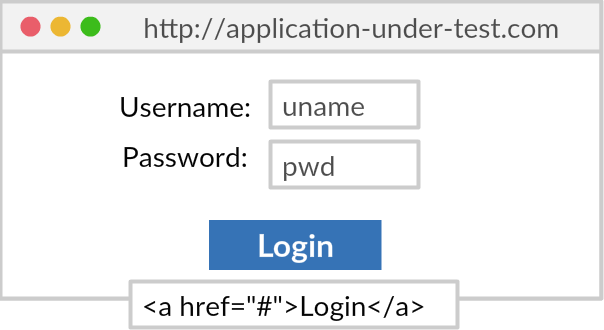
\includegraphics[width=5.6cm,height=2.8cm]{./Figures/newlogin}}
\vspace{-2mm}\subfigure[AUT version $V_{1}$]{\label{fig:3bnew}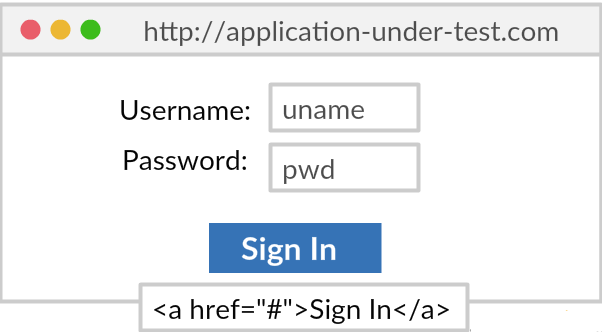
\includegraphics[width=5.6cm,height=2.8cm]{./Figures/newsignin}}
  \captionsetup{justification=justified,
singlelinecheck=false}
\caption{Evolution of the AUT from $V_{0}$ to $V_{1}$. Changing the GUI element locator for ``Login'' button breaks the fragile \texttt{loginTest}.}
\label{fig:3loginTest}
\end{figure} 

In order to explore this issue, let us revisit the introductory example which is repeated here in Figure \ref{fig:3loginTest}. In this example, the \texttt{loginTest} uses \texttt{link text} locator for locating the ``Login'' button: \begin{small}
\texttt{driver.findElement(By.linkText("Login")).click()}
\end{small}
As the AUT evolves from version $V_{0}$ to $V_{1}$, the hyperlink text for ``Login'' button changes to ``Sign In''. This change does not alter the functionality of the AUT, rather its look-and-feel. According to the definition of robustness which we have developed in the penultimate section (Definition \ref{test-case-robustness}), a robust test should be able to explore the same functionality of the AUT regardless of the changes in the look-and-feel of the AUT. However in this example, \texttt{loginTest} is broken due to the the structural change and it cannot explore the \texttt{login} functionality of the AUT anymore. 

If the \texttt{loginTest} in aforementioned example were to use a robust and structure independent locator, it might not have been susceptible to the renaming of ``Login'' button. Thus, choosing a suitable locator strategy plays a vital part for the robustness of the test. Each GUI locator differs in their characteristics such as availability and their susceptibility towards changes in GUI structure. A structure dependent locator is likely to be broken by minor changes in the application's GUI and needs to be repaired repeatedly if the AUT has frequent GUI changes. This process adds additional overhead in terms of the effort needed for the maintenance of the test-suite.  

To facilitate the maintenance of tests, the Page-object pattern (see Section \ref{page-object}) is helpful for the design of Selenium test-suites. This pattern provides a logical separation between the tests-code and the page-objects. Every time the test-suite needs to be repaired, such as changing the GUI element locator or changing the \texttt{wait} periods, developers can simply update the page-object as opposed to updating all tests. 

In this manner, the design strategy of a test-suite can also impact its maintenance effort. Intuitively, the two prominent building blocks where a test-suite needs to be frequently repaired are the GUI element locators and \texttt{wait} commands. A repairing procedure usually involves modifying different parts of these building blocks. A modification for a GUI element locator might involve changing its value; for instance, the \texttt{linkText("Login")} locator in above-mentioned example can be repaired to \texttt{linkText("Sign In")}. The \texttt{wait} commands can be modified to increase or decrease the waiting duration before performing certain action.

The \textit{effort} of maintaining a test-suite can be measured in terms of \textit{maintenance metrics}. The maintenance metrics of a test-suite indicate number of  GUI element locators and \texttt{wait} commands repaired during two subsequent revisions of the AUT. These metrics are formally expressed in Table \ref{rq3metrics}. 

This approach aims to assess how frequently are the test-suites maintained in comparison to the changes in the AUT. Our hypothesis is that every change to a test-suite's maintenance is intended to improve the quality of the test-suite. In other words, a test-suite is not repaired to harm or damage its robustness. If the test-suites do not need to be maintained to cope with minor revisions in the application, this can be an indication that the test-suite is relatively robust. If the developers know which of the presented maintenance metrics requires the least maintenance effort, they can write more robust tests by emphasizing the use of these metrics in the test design. 

\begin{center}
\begin{table}
\centering
\resizebox{13cm}{!}{
\begin{tabular}{l*{6}{l}r}
\hline
Maintenance Metric              &Description \\
\hline
% \hline
\textit{\#waitsRepaired}    & Number of \texttt{wait} commands repaired   \\
\hline
\textit{\#xpathRepaired}    & Number of \texttt{xpath} locators repaired\\
\textit{\#partialLinkTextRepaired}    & Number of \texttt{partial link text} locators repaired \\
\textit{\#classNameRepaired}    & Number of \texttt{class name} locators repaired \\
\textit{\#linkTextRepaired}    & Number of \texttt{link text} locators repaired  \\
\textit{\#nameRepaired}    & Number of \texttt{name} locators repaired \\
\textit{\#cssSelectorRepaired}    & Number of \texttt{css selector} locators repaired \\
\textit{\#tagNameRepaired}    & Number of \texttt{tag name} locators  repaired \\
\textit{\#idRepaired}    & Number of  \texttt{id} locators repaired \\
\hline
% \caption{Application Candidates}
\end{tabular}}
  \captionsetup{justification=justified,
singlelinecheck=false}
\caption{Overview of the test-suite maintenance metrics. The first part shows the number of repaired \texttt{wait} conditions, the second part shows the number of repaired GUI element locators.}
\label{rq3metrics}
\end{table}
\end{center}
